\documentclass{amsproc}
\usepackage{amssymb}
\usepackage{amsmath}
\usepackage{tikz}
\usepackage[siunitx, RPvoltages]{circuitikz}

\begin{document}

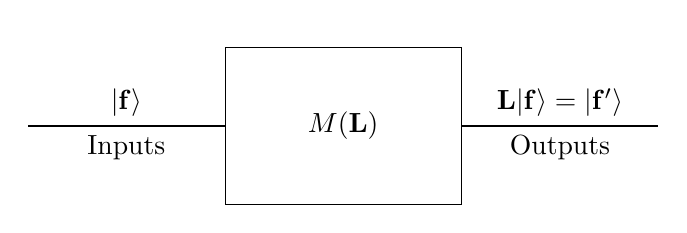
\begin{tikzpicture}
	\node[draw, rectangle, minimum width = 3 cm, minimum height = 2 cm] (fl) at (0,0) {$M({\bf L})$};
	\node[above] at (fl.north) {};
	\draw[-] (fl) -- node[above]{$|{\bf f}\rangle$} node[below]{Inputs} ++(-4,0);
	\draw[-] (fl) -- node[above]{${\bf L}|{\bf f}\rangle=|{\bf f}^{\prime}\rangle$} node[below]{Outputs} ++(4,0);
\end{tikzpicture}

\end{document}